\documentclass{article}
\usepackage{tikz}

\tikzset{% define a pic for the blocks, with the labels as arguments
   circnode/.style={circle, draw, minimum size=6mm, inner sep=0mm},
   pics/myblock/.style args={#1,#2}{
     code={\draw[thick,rounded corners](0,0) rectangle (1,4);
           \node at (0.5, 3.6) [circnode] {$#1_1$};
           \node at (0.5, 0.4) [circnode] {$#1_#2$};
           \foreach \y in {0.95,1.25,...,3.35} {
              \filldraw (0.5,\y) circle (1mm);
           }
      }
   },
   % and another pic for the bipartite graph
   pics/snare/.style = {
     code = { \foreach \y/\A in {0.4/A, 1.2/B, 2.8/C, 3.6/D} {
                 \coordinate (0\A) at (0,\y);
                 \coordinate (1\A) at (1,\y);
           }
           \draw(0A)--(1A)--(0B)--(1B)--(0C)--(1C)--(0D)--(1D)--(0B)
                    --(1C)--(0A)--(1D)--(0C)--(1A)--(0D)--(1D)--(0A)
                    --(1B);
     }
   }
}

\begin{document}

   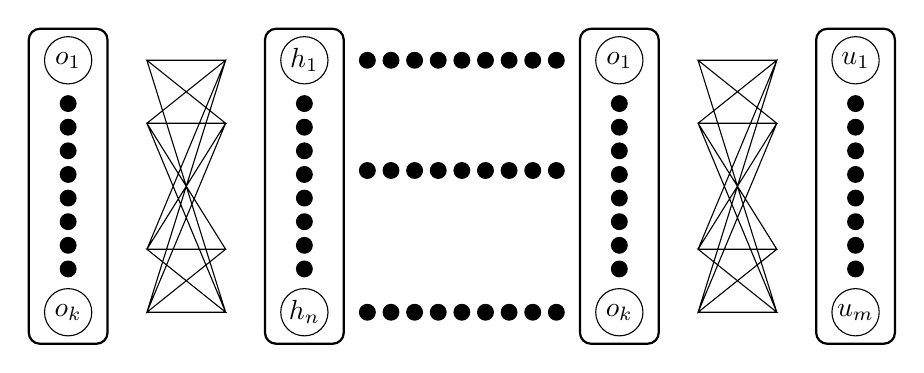
\begin{tikzpicture}
     \draw (0,0) pic{myblock={o,k}};
     \draw (1.5,0) pic{snare};
     \draw (3,0) pic{myblock={h,n}};
     \foreach \x in {4.3,4.6,...,6.9} {
         \foreach \y in {0.4, 2.2, 3.6} {
              \filldraw (\x,\y) circle (1mm);
         }
     }
     \draw (7,0) pic{myblock={o,k}};
     \draw (8.5,0) pic{snare};
     \draw (10,0) pic{myblock={u,m}};
   \end{tikzpicture}

\end{document}
